\documentclass[tikz]{standalone}
\usepackage{tikz}
\begin{document}
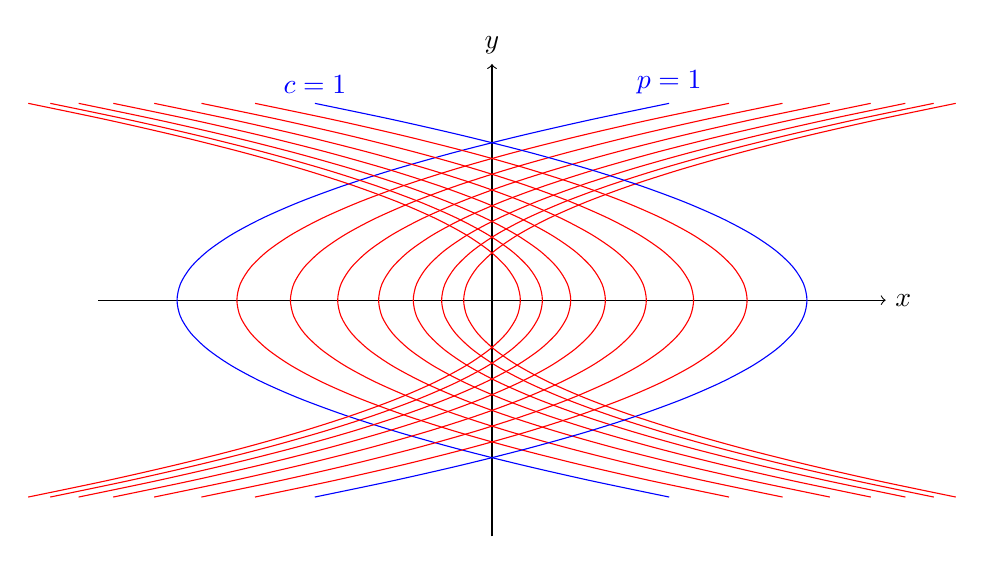
\begin{tikzpicture}
      \draw[->] (-5,0) -- (5,0) node[right] {$x$};
      \draw[->] (0,-3) -- (0,3) node[above] {$y$};
     % \draw[scale=0.5,domain=-3:3,smooth,variable=\x,blue] plot ({\x},{\x*\x});
      \foreach \temp in {0.3, 0.4, 0.5, 0.6, 0.7, 0.8, 0.9}{	      
     	 \draw[domain=-2.5:2.5,smooth,variable=\y,red]  plot ({\y*\y - 4*(\temp)*(\temp)},{\y});
     	 };
     	 \draw[domain=-2.5:2.5,smooth,variable=\y,blue]  plot ({\y*\y - 4},{\y}) node [above] {$p=1$};
     	
	  \foreach \temp in {-0.3, -0.4, -0.5, -0.6, -0.7, -0.8, -0.9}{	      
     	 \draw[domain=-2.5:2.5,smooth,variable=\y,red]  plot (-{\y*\y + 4*(\temp)*(\temp)},{\y});
     	 };
     	 \draw[domain=-2.5:2.5,smooth,variable=\y,blue]  plot (-{\y*\y + 4},{\y}) node [above] {$c=1$};
     	
    \end{tikzpicture}
\end{document}